\subsection{Co-Training with Vision-Language Datasets}
\begin{wrapfigure}{r}{0.3\linewidth}
   \centering
   \vspace{-0.7cm}
  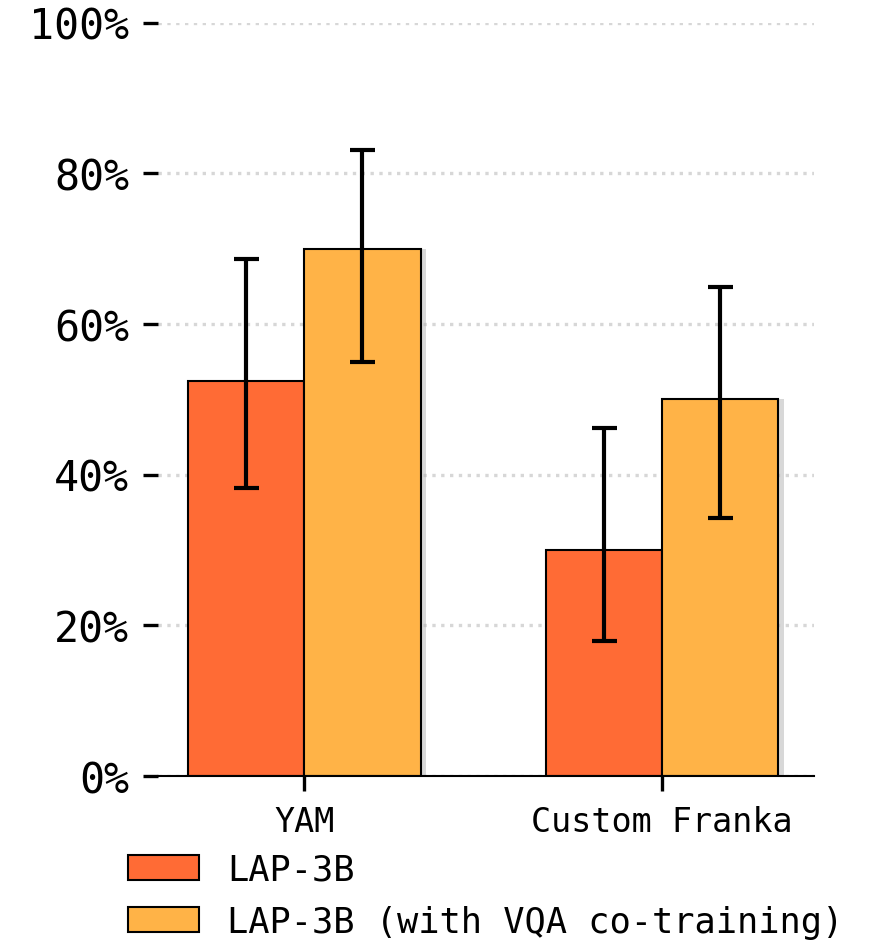
\includegraphics[width=\linewidth]{figures/fig8_cotrain.png}
  \caption{\textbf{VQA co-training} with a motion-prediction task improves cross-embodiment performance.}
  \label{fig:cotrain}
  \vspace{-0.5cm}
\end{wrapfigure}
We further investigate whether co-training with additional Visual-Question-Answering (VQA) tasks benefits \textsc{LAP-3B}.
We consider a motion-prediction task in which the model is prompted with two consecutive images and asked to predict the corresponding language-action describing the change between frames, analogous to an ``inverse dynamics'' prediction (Fig.~\ref{fig:teaser}, bottom left).
This co-training objective naturally bridges standard VQA-style supervision and our language-action prediction by sharing a unified, language-based output format.

We evaluate the resulting models on two embodiments, Custom Franka and YAM, with results shown in Fig.~\ref{fig:cotrain}.
Incorporating this motion-prediction VQA task leads to more precise action generation and improved spatial generalization, yielding higher success rates across embodiments.
In addition, co-training produces checkpoints that are easier to adapt to new tasks, enabling faster fine-tuning with fewer gradient steps and achieving higher final convergence performance (see Appendix~\ref{app:additional_results}).



\subsection{Scaling with Model Size}
% \par\medskip
\begin{wrapfigure}{r}{0.5\linewidth}
    \centering
    % \vspace{-1\baselineskip}
    \vspace{-0.4cm}
    \includegraphics[width=\linewidth]{figures/fig7_modelscaling.pdf}
    \caption{\textbf{Model scaling behavior of LAP compared to $\bm{\pi_{0.5}}$-replicated.}
    Left: Token validation loss, reported as percentage drop relative to the 4B model.
    Right: Continuous action validation loss of the diffusion-based action expert.
    \textsc{LAP-3B} improves consistently with scale, whereas the baseline saturates and degrades.}
    \label{fig:model-scaling}
    % \vspace{-20pt}
\end{wrapfigure}

We next investigate whether LAP benefits from increased model capacity, and whether its advantages persist in the large-model regime.

Using Gemma3 \cite{gemmateam2025gemma3technicalreport} as the VLM backbone, we train LAP models at 4B, 12B, and 27B parameter scales, and compare them against corresponding $\pi_{0.5}$-replicated variants, which represent the current state of the art in VLAs.

We evaluate two metrics on a held-out split comprising 2.5\% of the full data mixture: (i) token validation loss of the VLM backbone, and (ii) validation loss of the flow-matching-based action expert. For token validation loss, we report the percentage reduction relative to the 4B model, as absolute loss values are not directly comparable across different action representations. 

As shown in Fig.~\ref{fig:model-scaling}, LAP consistently attains lower validation loss across all model sizes and exhibits favorable scaling behavior, with performance improving monotonically as model capacity increases. In contrast, the $\pi_{0.5}$-replicated baseline shows early saturation and even degradation at larger scales. These results indicate that language-action supervision remains effective in the large-model regime and increasingly benefits from additional representational capacity.



